\documentclass{standalone}
\usepackage{tikz}
\usepackage{ctex,siunitx}
\usepackage{tkz-euclide}
\usepackage{amsmath}
\usetikzlibrary{patterns, calc}
\usetikzlibrary {decorations.pathmorphing, decorations.pathreplacing, decorations.shapes,}
\begin{document}
\small
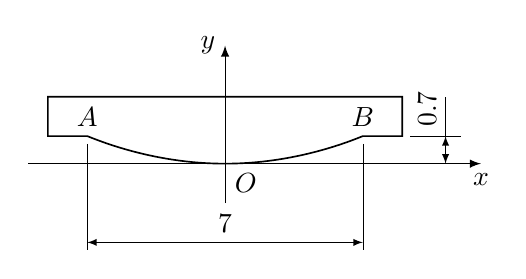
\begin{tikzpicture}[>=latex,scale=0.5]
  \draw[thin,->](-5,0)--(6.5,0)node[below]{$x$};
  \draw[thin,->](0,-1)--(0,3)node[left]{$y$};
  \draw[semithick](-4.5,0.7)--(-3.5,0.7)node[above]{$A$} parabola bend(0,0) (3.5,0.7) node[above]{$B$} --(4.5,0.7)--(4.5,1.7)--(-4.5,1.7)--cycle;
  \tkzDefPoints{0/0/O}
  \draw[very thin] (4.7,0.7)--(6,0.7)(5.6,0.7)--(5.6,1.7)(3.5,0.5)--(3.5,-2.2)(-3.5,0.5)--(-3.5,-2.2);
  \draw[very thin,<->](5.6,0)--(5.6,0.7)node[rotate=90,above right]{$0.7$};
  \draw[very thin,<->](-3.5,-2)--(3.5,-2)node[midway,above]{$7$};
  \tkzLabelPoints[below right](O)
\end{tikzpicture}
\end{document}